\chapter{Технологический раздел}
В данном разделе производится выбор средств реализации программного обеспечения, описываются типы и структуры данных, листинги кода, а так же будет продемонстрирован интерфейс программы.

\section{Выбор языка программирования и среды разработки}

Для реализации программного обеспечения был выбран язык C++ по нескольким причинам:
\begin{itemize}
	\item Поддерживает объектно-ориентированную парадигму программирования;
	\item Обладает достаточно высокой производительностью;
	\item Обладает широким набором функций из стандартной библиотеки, в том числе функция замера процессорного времени, которая будет использована в дальнейшем исследовании.
\end{itemize}

В качестве среды разработки был выбран Qt Creator. Он обладает всем необходимым функционалом для написания и отладки программ. Данная среда поставляется с фреймворком Qt, который будет использоваться для создания графического интерфейса программы.


\section{Выбор структур данных}
В данной работе необходимо создать следующие структуры данных:

\begin{itemize}
	\item Структура, характеризующая перемещение модели;
	\item Структура, характеризующая вращение модели;
	\item Структура, характеризующая масштабирование модели;
	\item Класс, описывающий точку;
	\item Класс, описывающий точки;
	\item Структура, описывающая ребро;
	\item Класс, описывающий ребра;
	\item Структура, описывающая грань;
	\item Класс, описывающий грани;
	\item Класс, описывающий фигуру;
	\item Класс, описывающий отрисовываемое полотно;
	\item Класс, необходимый для взаимодействия пользователя с программой.
\end{itemize}


\section{Структура программы}
На рисунке~\ref{fig:uml_programm} представлена структура программы в виде UML-диаграммы.

\begin{figure}[H]
	\centering
	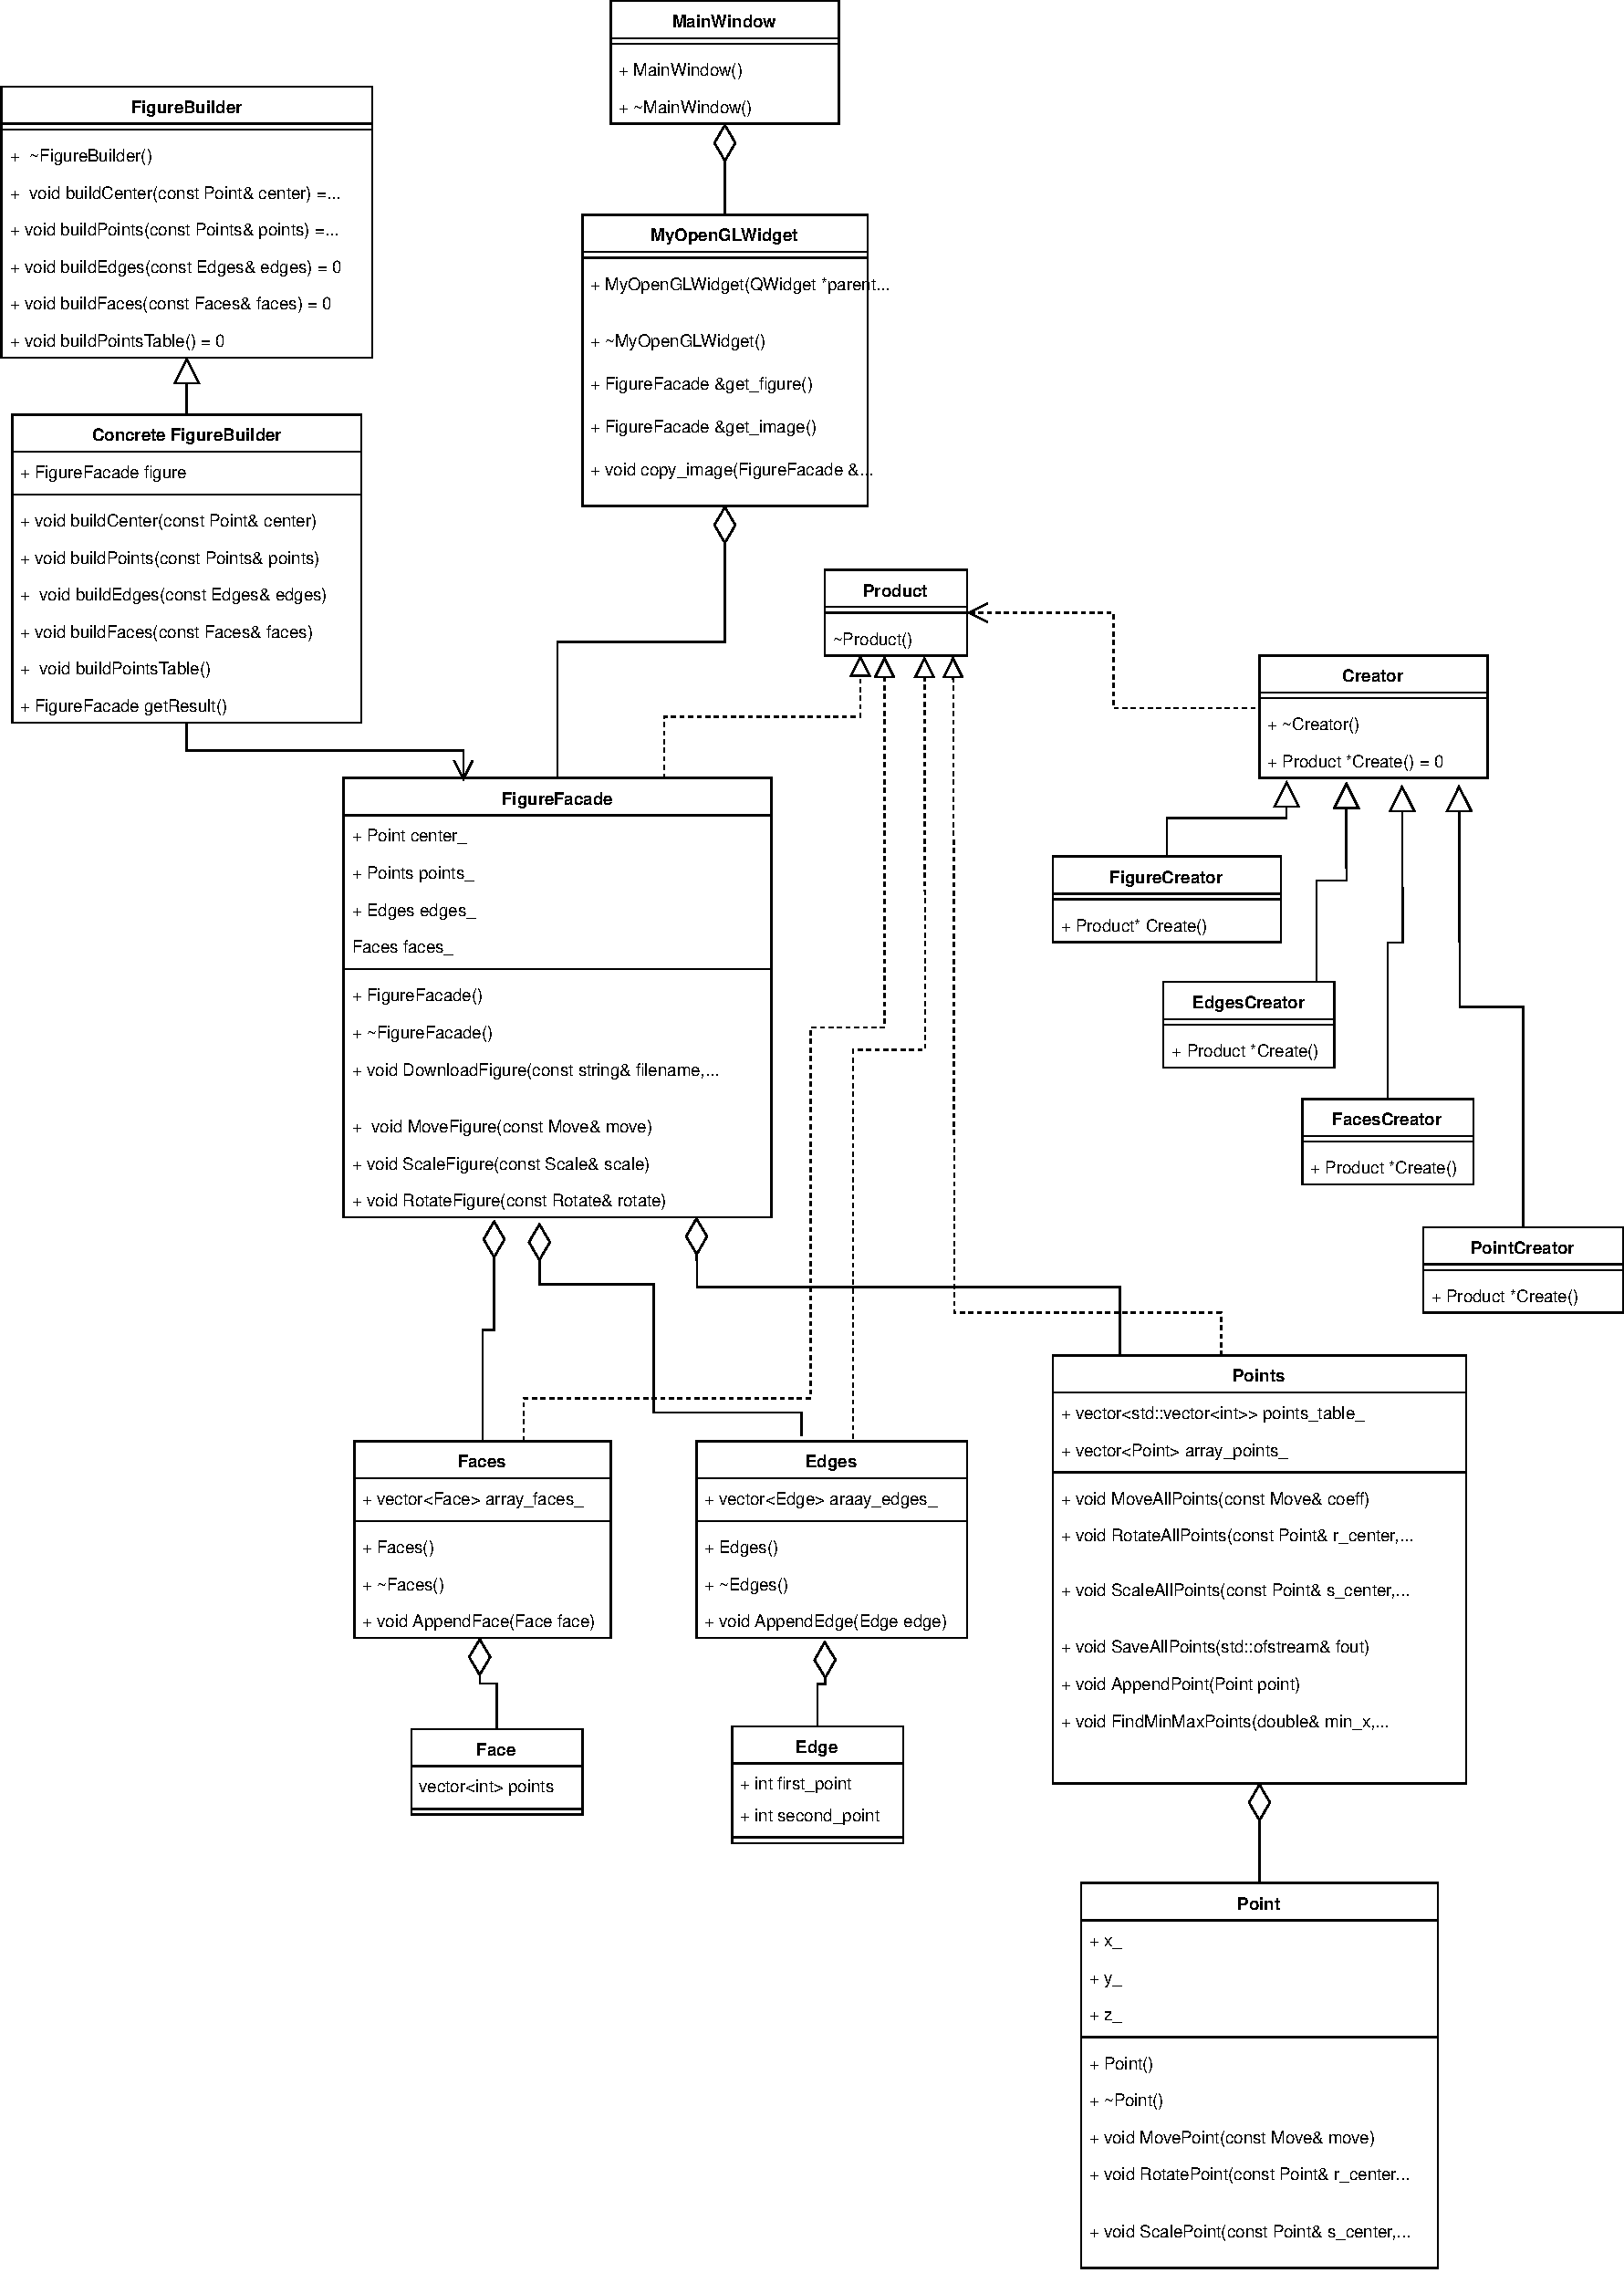
\includegraphics[scale=0.54]{images/programm.pdf}
	\caption{Структура программы}
	\label{fig:uml_programm}
\end{figure}

\newpage

\section{Реализация алгоритмов}
Реализация алгоритма создания фигуры и считывания ее вершин и ребер из .obj файла предоставлена на листингах~\ref{lst:create_load_figure.cpp} -- \ref{lst:exist_edge.cpp}.
Необходимо отметить, что очередное ребро не просто заносится в список. 
Сначала проверяется его наличие (см. листинги~\ref{lst:read_faces.cpp} -- \ref{lst:faces_to_edges.cpp}).
Так же для построения фигуры используется паттерн строитель – так код становится логически проще.
За выделение памяти отвечает фабричный метод.

\includelistingpretty
{create_load_figure.cpp}
{c++}
{Создание и загрузка фигуры}

\includelistingpretty
{read_vertices.cpp}
{c++}
{Чтение вершин из файла}

\includelistingpretty
{read_faces.cpp}
{c++}
{Чтение граней из файла}

\includelistingpretty
{faces_to_edges.cpp}
{c++}
{Получение ребер из граней}

\includelistingpretty
{build_points_table.cpp}
{c++}
{Заполнение таблицы смежности для точек}

\includelistingpretty
{exist_edge.cpp}
{c++}
{Проверка ребра на наличие в таблице смежности}


Реализация алгоритма отображения сцены предоставлена на листингах ~\ref{lst:paint_gl.cpp} -- \ref{lst:draw_faces.cpp}. 
Здесь алгоритм Z-буфера и настройка камеры и света реализованы средствами OpenGL.
Так повышается производительность программы, ведь методы OpenGL используют аппаратное ускорение (многие методы выполняются на графическом процессоре) и параллелизм при обработке вершин. 
Настройка камеры происходит относительно размеров фигуры. 
Так она всегда находится в области видимости камеры.

\includelistingpretty
{paint_gl.cpp}
{c++}
{Инициализация и перерисовка сцены}

\includelistingpretty
{init_camera.cpp}
{c++}
{Настройка камеры и света}

\includelistingpretty
{draw_vertices.cpp}
{c++}
{Отрисовка вершин}

\includelistingpretty
{draw_edges.cpp}
{c++}
{Отрисовка ребер}

\includelistingpretty
{draw_faces.cpp}
{c++}
{Отрисовка граней}

Реализация морфинга двух фигур представлена на листинге~\ref{lst:morph.cpp}.

\includelistingpretty
{morph.cpp}
{c++}
{Морфинг двух фигур}


\section{Интерфейс программы}

Программа предоставляет следующий графический интерфейс (см. рис. 3.1). 
При первом запуске все виджеты имеют значения по умолчанию, при следующих запусках программы значения сохраняются.
Пользователь видит сцену (справа), виджеты (слева) и меню (сверху). 
С помощью меню он может:

\begin{enumerate}
	\item Загружать новую модель.
	Если модель уже была на сцене, начнется процесс морфинга.
	\item Менять отрисовку с помощью виджетов:
	
	\begin{itemize}
		\item Перемещать модель вдоль осей;
		\item Поворачивать модель вокруг осей;
		\item Масштабировать модель;
		\item Изменять размер ребер (видно при морфинге);
		\item Изменять размер вершин (видно при морфинге);
		\item Изменять тип вершин (видно при морфинге);
		\item Изменять тип ребер (видно при морфинге);
		\item Перемещать камеру;
		\item Перемещать источник света.
	\end{itemize}
\end{enumerate}

%Тут надо будет вставить рисунки


\section*{Выводы из технологического раздела}

В этом разделе были выбраны средства реализации программы и необходимые структуры данных, описана структура программы, а также предоставлена реализация алгоритмов и пользовательский интерфейс.
